\documentclass{article}
\usepackage[margin=1in]{geometry}
\usepackage[linesnumbered,ruled,vlined]{algorithm2e}
\usepackage{amsfonts}
\usepackage{amsmath}
\usepackage{amssymb}
\usepackage{amsthm}
\usepackage{enumitem}
\usepackage{fancyhdr}
\usepackage{hyperref}
\usepackage{minted}
\usepackage{multicol}
\usepackage{pdfpages}
\usepackage{standalone}
\usepackage[many]{tcolorbox}
\usepackage{tikz-cd}
\usepackage{transparent}
\usepackage{xcolor}
% \tcbuselibrary{minted}

\author{Nathan Solomon}

\newcommand{\fig}[1]{
    \begin{center}
        \includegraphics[width=\textwidth]{#1}
    \end{center}
}

% Math commands
\renewcommand{\d}{\mathrm{d}}
\DeclareMathOperator{\id}{id}
\DeclareMathOperator{\im}{im}
\DeclareMathOperator{\proj}{proj}
\DeclareMathOperator{\Span}{span}
\DeclareMathOperator{\Tr}{Tr}
\DeclareMathOperator{\tr}{tr}
\DeclareMathOperator{\ad}{ad}
\DeclareMathOperator{\ord}{ord}
%%%%%%%%%%%%%%% \DeclareMathOperator{\sgn}{sgn}
\DeclareMathOperator{\Aut}{Aut}
\DeclareMathOperator{\Inn}{Inn}
\DeclareMathOperator{\Out}{Out}
\DeclareMathOperator{\stab}{stab}

\newcommand{\N}{\ensuremath{\mathbb{N}}}
\newcommand{\Z}{\ensuremath{\mathbb{Z}}}
\newcommand{\Q}{\ensuremath{\mathbb{Q}}}
\newcommand{\R}{\ensuremath{\mathbb{R}}}
\newcommand{\C}{\ensuremath{\mathbb{C}}}
\renewcommand{\H}{\ensuremath{\mathbb{H}}}
\newcommand{\F}{\ensuremath{\mathbb{F}}}

\newcommand{\E}{\ensuremath{\mathbb{E}}}
\renewcommand{\P}{\ensuremath{\mathbb{P}}}

\newcommand{\es}{\ensuremath{\varnothing}}
\newcommand{\inv}{\ensuremath{^{-1}}}
\newcommand{\eps}{\ensuremath{\varepsilon}}
\newcommand{\del}{\ensuremath{\partial}}
\renewcommand{\a}{\ensuremath{\alpha}}

\newcommand{\abs}[1]{\ensuremath{\left\lvert #1 \right\rvert}}
\newcommand{\norm}[1]{\ensuremath{\left\lVert #1\right\rVert}}
\newcommand{\mean}[1]{\ensuremath{\left\langle #1 \right\rangle}}
\newcommand{\floor}[1]{\ensuremath{\left\lfloor #1 \right\rfloor}}
\newcommand{\ceil}[1]{\ensuremath{\left\lceil #1 \right\rceil}}
\newcommand{\bra}[1]{\ensuremath{\left\langle #1 \right\rvert}}
\newcommand{\ket}[1]{\ensuremath{\left\lvert #1 \right\rangle}}
\newcommand{\braket}[2]{\ensuremath{\left.\left\langle #1\right\vert #2 \right\rangle}}

\newcommand{\catname}[1]{{\normalfont\textbf{#1}}}

\newcommand{\up}{\ensuremath{\uparrow}}
\newcommand{\down}{\ensuremath{\downarrow}}

% Custom environments
\newtheorem{thm}{Theorem}[section]

\definecolor{probBackgroundColor}{RGB}{250,240,240}
\definecolor{probAccentColor}{RGB}{140,40,0}
\newenvironment{prob}{
    \stepcounter{thm}
    \begin{tcolorbox}[
        boxrule=1pt,
        sharp corners,
        colback=probBackgroundColor,
        colframe=probAccentColor,
        borderline west={4pt}{0pt}{probAccentColor},
        breakable
    ]
    \color{probAccentColor}\textbf{Problem \thethm.} \color{black}
} {
    \end{tcolorbox}
}

\definecolor{exampleBackgroundColor}{RGB}{212,232,246}
\newenvironment{example}{
    \stepcounter{thm}
    \begin{tcolorbox}[
      boxrule=1pt,
      sharp corners,
      colback=exampleBackgroundColor,
      breakable
    ]
    \textbf{Example \thethm.}
} {
    \end{tcolorbox}
}

\definecolor{propBackgroundColor}{RGB}{255,245,220}
\definecolor{propAccentColor}{RGB}{150,100,0}
\newenvironment{prop}{
    \stepcounter{thm}
    \begin{tcolorbox}[
        boxrule=1pt,
        sharp corners,
        colback=propBackgroundColor,
        colframe=propAccentColor,
        breakable
    ]
    \color{propAccentColor}\textbf{Proposition \thethm. }\color{black}
} {
    \end{tcolorbox}
}

\definecolor{thmBackgroundColor}{RGB}{235,225,245}
\definecolor{thmAccentColor}{RGB}{50,0,100}
\renewenvironment{thm}{
    \stepcounter{thm}
    \begin{tcolorbox}[
        boxrule=1pt,
        sharp corners,
        colback=thmBackgroundColor,
        colframe=thmAccentColor,
        breakable
    ]
    \color{thmAccentColor}\textbf{Theorem \thethm. }\color{black}
} {
    \end{tcolorbox}
}

\definecolor{corBackgroundColor}{RGB}{240,250,250}
\definecolor{corAccentColor}{RGB}{50,100,100}
\newenvironment{cor}{
    \stepcounter{thm}
    \begin{tcolorbox}[
        enhanced,
        boxrule=0pt,
        frame hidden,
        sharp corners,
        colback=corBackgroundColor,
        borderline west={4pt}{0pt}{corAccentColor},
        breakable
    ]
    \color{corAccentColor}\textbf{Corollary \thethm. }\color{black}
} {
    \end{tcolorbox}
}

\definecolor{lemBackgroundColor}{RGB}{255,245,235}
\definecolor{lemAccentColor}{RGB}{250,125,0}
\newenvironment{lem}{
    \stepcounter{thm}
    \begin{tcolorbox}[
        enhanced,
        boxrule=0pt,
        frame hidden,
        sharp corners,
        colback=lemBackgroundColor,
        borderline west={4pt}{0pt}{lemAccentColor},
        breakable
    ]
    \color{lemAccentColor}\textbf{Lemma \thethm. }\color{black}
} {
    \end{tcolorbox}
}

\definecolor{proofBackgroundColor}{RGB}{255,255,255}
\definecolor{proofAccentColor}{RGB}{80,80,80}
\renewenvironment{proof}{
    \begin{tcolorbox}[
        enhanced,
        boxrule=1pt,
        sharp corners,
        colback=proofBackgroundColor,
        colframe=proofAccentColor,
        borderline west={4pt}{0pt}{proofAccentColor},
        breakable
    ]
    \color{proofAccentColor}\emph{\textbf{Proof. }}\color{black}
} {
    \qed \end{tcolorbox}
}

\definecolor{noteBackgroundColor}{RGB}{240,250,240}
\definecolor{noteAccentColor}{RGB}{30,130,30}
\newenvironment{note}{
    \begin{tcolorbox}[
        enhanced,
        boxrule=0pt,
        frame hidden,
        sharp corners,
        colback=noteBackgroundColor,
        borderline west={4pt}{0pt}{noteAccentColor},
        breakable
    ]
    \color{noteAccentColor}\textbf{Note. }\color{black}
} {
    \end{tcolorbox}
}


\fancyhf{}
\setlength{\headheight}{24pt}

\date{\today}
\title{Math 115B Homework \#3}

\begin{document}
\maketitle

\begin{prob}
\end{prob}
We know similar matrices have the same eigenvalues (with the same multiplicities), and since a characteristic polynomial can be uniquely determined from the eigenvalues and their multiplicities, $A$ and $D$ must have the same characteristic polynomial. The matrix $D$ can be written as
\[ D = \begin{bmatrix}
    \lambda_1 & 0 \\
    0 & \lambda_2
\end{bmatrix}, \]
so its characteristic polynomial is $p_D(x) = (\lambda_1 - x)(\lambda_2 - x) = p_A(x)$. When we plug $A$ into that polynomial, we get
\begin{align*}
    p_A(A) &= (\lambda_1 - A)(\lambda_2 - A) \\
           &= \lambda_1 \lambda_2 - \lambda_1 A - \lambda_2 A + A^2 \\
           &= \lambda_1 \lambda_2 - \lambda_1 QDQ^{-1} - \lambda_2 QDQ^{-1} + QD^2Q^{-1} \\
           &= Q \left( \lambda_1 \lambda_2 I - \lambda_1 D - \lambda_2 D + D^2 \right) Q^{-1} \\
           &= Q \begin{bmatrix}
               \lambda_1 \lambda_2 - \lambda_1^2 - \lambda_2 \lambda_1 + \lambda_1^2 & 0 \\
               0 & \lambda_1 \lambda_2 - \lambda_1 \lambda_2 - \lambda_2^2 + \lambda_2^2
           \end{bmatrix} Q^{-1} \\
           &= 0.
\end{align*}

\bigskip
\par
\begin{prob}
\end{prob}
\begin{enumerate}[label=(\alph*)]
    \item The first few powers of $T$ acting on $v$ are
        \[ T^0 v = \begin{bmatrix}
            1 \\
            0 \\
            0 \\
            0
        \end{bmatrix}, T^1 v = \begin{bmatrix}
            1 \\
            0 \\
            1 \\
            1
        \end{bmatrix}, T^2 v = \begin{bmatrix}
            1 \\
            -1 \\
            2 \\
            2
        \end{bmatrix}, T^3 v = \begin{bmatrix}
            0 \\
            -3 \\
            3 \\
            3
        \end{bmatrix}, \dots \]
        Those first 3 vectors are clearly linearly independent, but by induction, we know that the last two components of $T^n(v)$ (that is, $e_3^* T^n v$ and $e_4^* T^n v$) will always be the same, so the dimension of the $T$-cyclic subspace generated by $v$ cannot be more than 3. Therefore, $ \left( v, Tv, T^2v \right) $ is a basis for that subspace.
    \item $v=x^2$ and $Tv=2$, and for any $n > 1, T^n v=0$. Therefore $ (v, Tv)$ is a basis for the $T$-cyclic subspace generated by $v$.
    \item $Tv=v$, so $T^nv=v$ for any $n$, which means the singleton $(v)$ is a basis for the $T$-cyclic subspace generated by $v$.
    \item
        \[ v = \begin{bmatrix}
            0 & 1 \\
            1 & 0
        \end{bmatrix}, Tv = \begin{bmatrix}
            1 & 1 \\
            2 & 2
        \end{bmatrix}, T^2 v = \begin{bmatrix}
            3 & 3 \\
            6 & 6
        \end{bmatrix}, \dots \]
        We can see that $v$ and $Tv$ are linearly independent, but $T^2 v = 3 Tv$, which means $T^n v \propto T v$ whenever $n > 0$. Therefore the $T$-cyclic subspace generated by $v$ is 2-dimensional, so $(v, Tv)$ is a basis for it.
\end{enumerate}

\bigskip
\par
\begin{prob}
\end{prob}
\begin{enumerate}[label=(\alph*)]
    \item In the basis I chose in the previous problem, $T|_W$ is described by the matrix
        \[ T|_W = \begin{bmatrix}
            0 & 0 & 0 \\
            1 & 0 & -3 \\
            0 & 1 & 3
        \end{bmatrix} \]
        because $T^3 v = 3 T^2 v - 3 T v$. Therefore the characteristic polynomial is
        \[ p(\lambda) = (-\lambda)(-\lambda)(3-\lambda) - (\lambda)(-3)(1) = - \lambda^3 + 3 \lambda^2 + 3 \lambda. \]
    \item In the basis I chose in the previous problem, $T|_W$ is described by the matrix
        \[ T|_W = \begin{bmatrix}
            0 & 0 \\
            1 & 0
        \end{bmatrix}, \]
        so the characteristic polynomial is $p(\lambda) = \lambda^2$.
    \item $T|_W$ is just the identity matrix, so its characteristic polynomial is $p(\lambda) = 1 - \lambda$.
    \item In the basis I chose in the previous problem, $T|_W$ is described by the matrix
        \[ T|_W = \begin{bmatrix}
            0 & 0 \\
            1 & 3
        \end{bmatrix}, \]
        so the characteristic polynomial is $p(\lambda) = (-\lambda)(3-\lambda)=\lambda^2-3\lambda$.
\end{enumerate}


\bigskip
\par
\begin{prob}
\end{prob}
Surjective is equivalent to having a right inverse, and injective is equivalent to having a left inverse
\begin{enumerate}[label=(\alph*)]
    \item $T$ is surjective iff it has a right inverse, meaning there exists a linear map $T^{-1}: W \rightarrow V$ such that $T \circ T^{-1} = I_W$. The dual of that is $(T \circ T^{-1})^* = I_{w^*}$, and by the definition of a dual, the dual of $(T \circ T^{-1}) : W \rightarrow W$ is the linear functional which maps $w^* \in W^*$ to $w^* \circ T \circ T^{-1}$, which can also be written as
        \[ W^* \circ T \circ T^{-1} = (T^{-1})^* \circ (w^* \circ T) = (T^{-1})^* \circ (T^* \circ w^*) = ((T^{-1})^* \circ T^*) w^*. \]
        Therefore, the dual of $(T \circ T^{-1})$ is $(T^{-1})^* \circ T^*$, and vice versa. $(T^{-1})^*$ is a left inverse of $T^*$, and if we did not already know $T$ was surjective, we could have instead defined $T^{-1}$ such that $(T^{-1})^*$ is a left inverse of $T^*$. Thus, a right inverse of $T$ exists iff a left inverse of $T^*$ exists. That's equivalent to saying $T$ is surjective iff $T^*$ is injective.
    \item This can be derived from the statement I proved in part (a) by replacing the symbols $T^*$ with $T$, $V^*$ with $W$, and $W^*$ with $V$. Then the statement becomes ``$T^*$ is surjective iff $T^{**}$ is injective", but we know $T^{**}$ is indistinguishable from $T$.
\end{enumerate}


\bigskip
\par
\begin{prob}
\end{prob}
The characteristic polynomial of $A$ is equal to
\[ p_A(\lambda) = \det \left( \begin{bmatrix}
        -\lambda & 0 & \cdots & 0 & -a_0 \\
        1 & -\lambda & \cdots & 0 & -a_1 \\
        0 & 1 & \cdots & 0 & -a_2 \\
        \vdots & \vdots & \ddots & \vdots & \vdots \\
        0 & 0 & \cdots & -\lambda & -a_{d-2} \\
        0 & 0 & \cdots & 1 & -a_{d-1}-\lambda \\
\end{bmatrix} \right)  \]
If $d=1$, that matrix has only one entry, which is $-a_0-\lambda$, therefore the characteristic polynomial is $p_A(\lambda)=(-1)^1(a_0+\lambda)$, so the statement we want to prove is true.
\par
If the statement is true for $d-1$, then consider the submatrix of $A-\lambda I$ with the first row and column removed. The determinant of that matrix is
\[ (-1)^{d-1}(a_1+a_2 \lambda + \cdots + a_{d-1} \lambda^{d-2} + \lambda^{d-1}). \]
Now we want to calculate the determinant of the entire matrix $A-\lambda I$, whose first row is all zeros, except for the leftmost entry, which is $-\lambda$, and the rightmost entry, which is $a_0$. Using the general, explicit formula for the determinant of a matrix, the determinant of $A-\lambda I$ is then
\[ (-\lambda) \cdot (-1)^{d-1}(a_1+a_2 \lambda + \cdots + a_{d-1} \lambda^{d-2} + \lambda^{d-1}) + (-a_0)(1)(-1)^{d-1} = (-1)^d (a_0+a_1 \lambda + \cdots + a_{d-1} \lambda + \lambda^d). \]
That means the statement is also true for $d$, so by induction, it is true whenever $d$ is a positive integer.

\bigskip
\par
\begin{prob}
\end{prob}
Let $W$ be any $T$-invariant subspace of $V$.
\begin{enumerate}[label=(\alph*)]
    \item Let $p_W$ be the characteristic polynomial of $T$ restricted to $W$, and let $p_V$ be the characteristic polynomial of $T$. We know that $p_W$ divides $p_V$, meaning there exists a polynomial $q$ such that $p_V = q \cdot p_W$. If $p_W$ does not split, then neither does $p_V$. Conversely, if $p_V$ splits, then so does $p_W$.
    \item If $p_V$ splits, then so does $p_W$, which means $T|_W$ has at least one eigenvalue. Since we assumed $W$ is nonzero, that implies $W$ has at least one eigenvector.
\end{enumerate}


\bigskip
\par
\begin{prob}
\end{prob}
\begin{enumerate}[label=(\alph*)]
    \item \textbf{Base case:} if $d=1$, then $\sum_{i=1}^d v_i \in W$ implies $v_1 \in W$.
        \par
        \textbf{Inductive step:} if this statement is true for $d-1$, then consider whether it's true for $d$. Suppose $v_1, v_2, \dots, v_d$ are eigenvectors of $T$ with distinct eigenvalues, and $\sum_{i=1}^d v_i \in W$. By my assumption, $u := \sum_{i=1}^{d-1} v_i$ is in $W$, and $u+v_d$ is in $W$, which means $(u+v_d)-u=v_d$ is in $W$.
        \par
        By induction, the statement is true for any positive integer $d$.
    \item
\end{enumerate}

\bigskip
\par
\begin{prob}
\end{prob}

\bigskip
\par
\begin{prob}
\end{prob}
The Cayley-Hamilton theorem says that $A^n$ is a linear combination of $I, A, A^2, \dots, A^{n-1}$. By induction, we also know that $A^m$ is a linear combination of $I, A, A^2, \dots, A^{n-1}$ whenever $m \geq n$, so
\begin{align*}
    \Span \left( \left\{ I, A, A^2, \dots \right\} \right) &= \Span \left( \left\{ I, A, A^2, \dots, A^{n-1} \right\} \right) \\
    \dim \left( \Span \left( \left\{ I, A, A^2, \dots \right\} \right) \right) &= \dim \left( \Span \left( \left\{ I, A, A^2, \dots, A^{n-1} \right\} \right) \right) \leq n.
\end{align*}

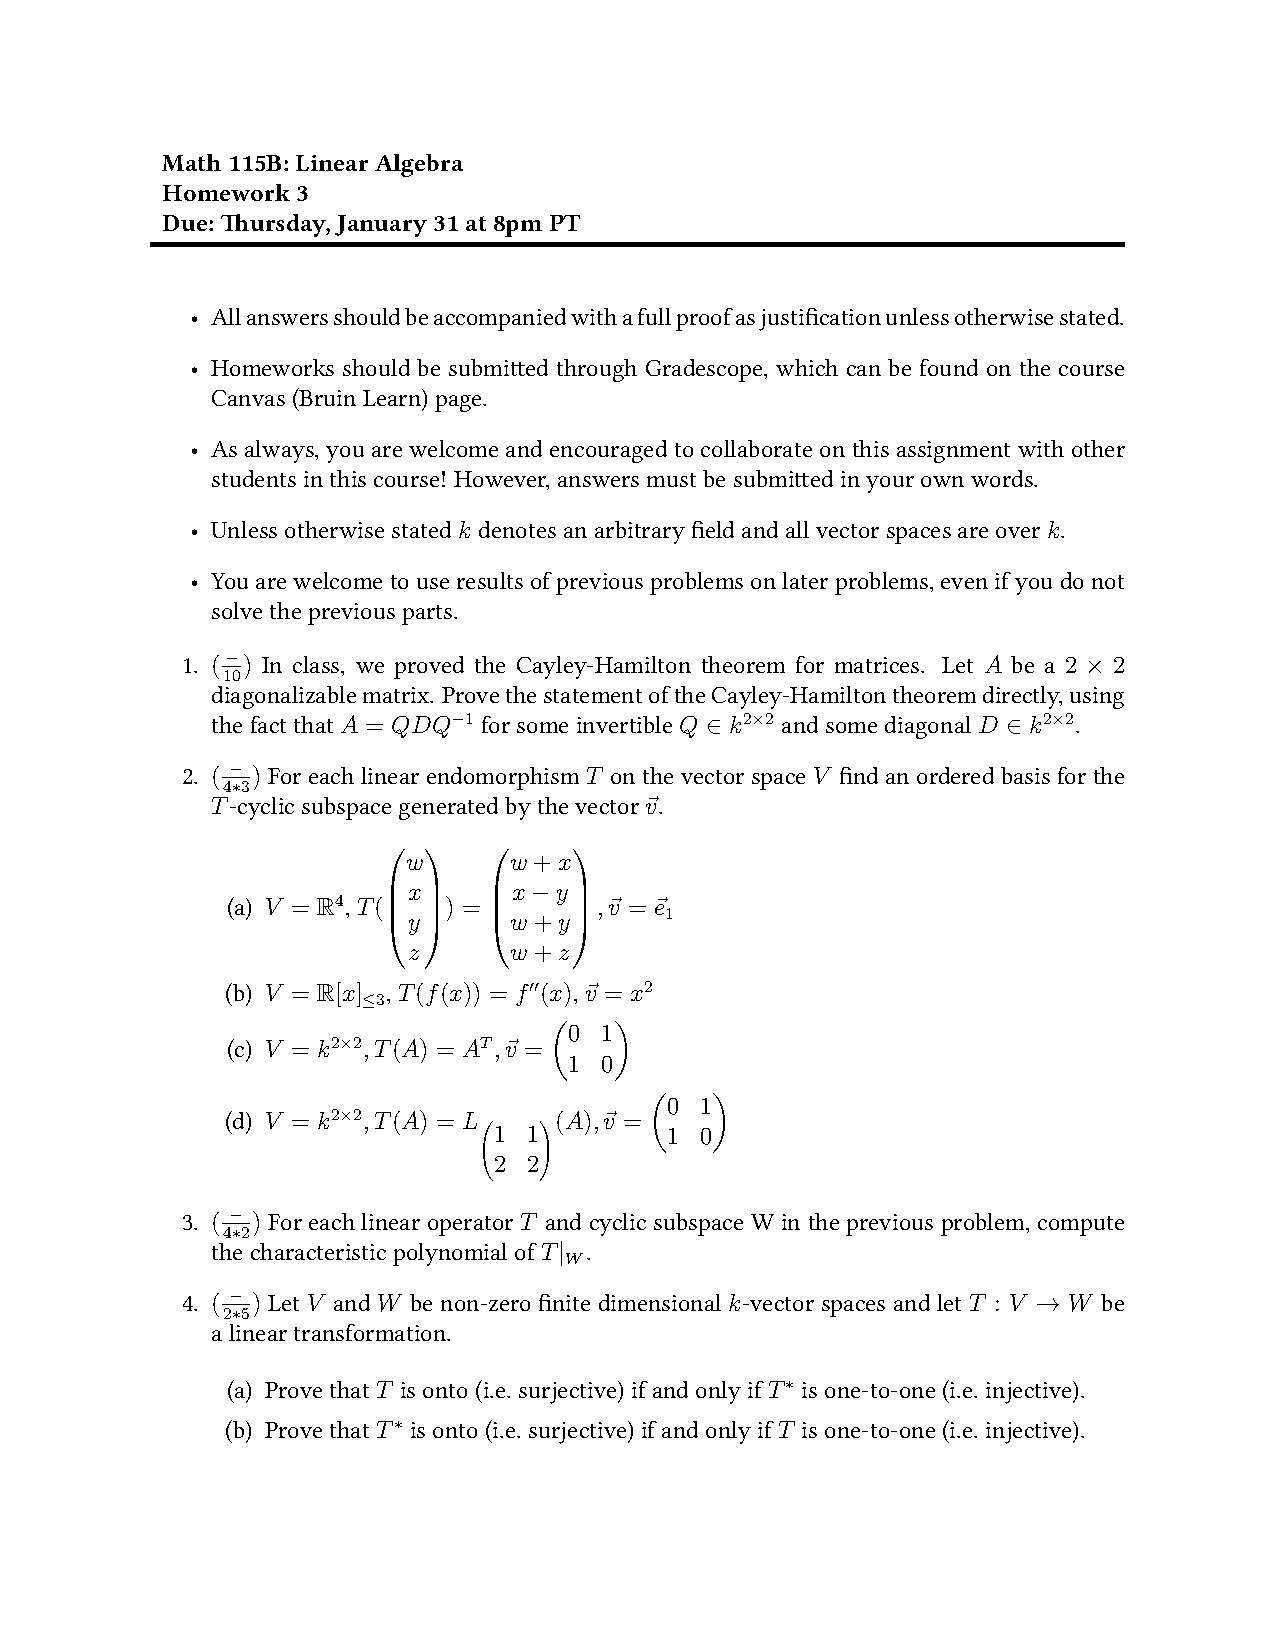
\includepdf[pages=-]{assignment.pdf}

\end{document}
